\lstset{style=ang}
\section{Introduction}
Angort\footnote{The name is an entirely random pair of syllables,
it has no significance.}
is a stack-based concatenative programming language with some
functional features. The language has grown from a simple Forth-like
core over time, and has been used primarily for robot control on
an ExoMars rover locomotion prototype.

This is an extremely brief introduction to the language. It may
be useful for readers unfamiliar with this style of programming
to look into Forth, which is an older, more primitive (but faster and
smaller) language from which much of the syntax of Angort was
borrowed.

It combines the power and ease of a modern dynamic language with
the convenience of a Forth-like language for controlling robots in
real time. For example, on our rover we have the following definitions
in the startup file:

\begin{lstlisting}
# define a constant "wheels" holding a range from 1-6 inclusive

range 1 7 const wheels

# define a new word "d" with a single parameter "speed"

:d [speed:]

    # set a help text for this word

    :"(speed --) set speed of all drive motors"
    
    # for each wheel, set the required speed to the value
    # of the parameter
    
    wheels each {
        ?speed i!drive
    }
;

# slightly more complex word for steering

:t [angle:]
    :"(angle --) turn front wheels one way, back wheels opposite way"
    
    ?angle dup 1!steer 2!steer
    0 0 3!steer 4!steer
    ?angle neg dup 5!steer 6!steer
;

# define a word to stop the rover by setting all speeds to zero

:s 0 d;

\end{lstlisting}
Once these words are defined we can steer the robot in real time with
commands like:
\begin{v}
2500 d
30 t
s
\end{v}
These will set the rover speed to 2500, turn it to 30 degrees, and stop
it respectively. We can also directly type things like:
\begin{v}
wheels each { i dactual .}
\end{v}
which will print the actual speeds of all the wheels.
It's also possible to perform some functional programming with
anonymous functions:
\begin{v}
:sum |list:| 0 ?list (+) reduce;
\end{v}
will allow us to sum a list and print the results:
\begin{v}
[1,2,3,4,5] sum .
\end{v}
or even:
\begin{v}
1 1001 range (dup*) map sum .
\end{v}
to print the sum of the squares of the first 1000 integers.
As can be seen, Angort is a very terse language.

In the examples given so far, words such as \texttt{dactual},
\texttt{!drive} and \texttt{?drive} are links to native C++ code: it
is very easy to interface Angort with C++.

\subsection{Downloading and building Angort}
Angort can be downloaded from \url{https://github.com/jimfinnis/angort} .
Once downloaded it, can be built with the following commands (from
inside the top-level Angort directory):
\begin{v}
mkdir build
cd build
cmake ..
make
\end{v}
This is for a Linux machine
with CMake and the \texttt{readline} development libraries. The standard
interpreter will then be installed in \texttt{cli/angortcli} .

\section{Getting started: immediate mode}
Running the interpreter will give a prompt:
\begin{v}
1|0>
\end{v}
The two numbers are the number of garbage-collectable objects in the
system and the number of items on the stack, respectively.
The interpreter is in ``immediate mode'', as opposed to ``compilation
mode'' --- any words entered will be compiled to bytecode and run when
enter is pressed,
rather than being added to a word definition.

In this mode, control constructs like
\texttt{if...else...then} or loops cannot span more than one
line. This is because such structures can only operate within a single 
bytecode block, and the current block is closed and run at the end of each
line in immediate mode. Inside a word definition this rule does not apply.


\section{The stack}
Angort is a stack-based language: there is a single stack containing
values, and most words change the contents
of the stack in some way. For example,
\begin{v}
3
\end{v}
by itself will just put the value 3 on the stack. Then
\begin{v}
.
\end{v}
will pop the value from the top of the stack and print it.
\begin{v}
3 4 + .
\end{v}
will push 3 and 4 onto the stack, then add them together replacing them
with 7, and then print the 7. More complex expressions are built 
out of sequences of operations on the stack. For example, the expression
\[
\sin(5+32+\sqrt{43 \times 12})
\]
would be written as
\begin{v}
43 12 * sqrt 32 + 5 + sin
\end{v}
Converting expressions into this so-called \emph{reverse Polish notation}
is a little difficult at first, but rapidly becomes second
nature\footnote{Most old calculators work using RPN, and quite a few
of the more powerful programmables still do.}

\section{Defining new words}
New words are defined with code of the form
\begin{v}
:wordname ... ;
\end{v}
A simple example is:
\begin{v}
:square dup *;
\end{v}
This will define a word \texttt{square} which will duplicate
the value on top of the stack, multiply the top two values
(effectively squaring the number\footnote{This will produce
an error if the value is not a number.}) and exit, leaving the
squared number on the stack. This can then be used thus:
\begin{v}
3 square 4 square + .
\end{v}
which will print 25, i.e. $3^2+4^2$.
While defining a word, Angort is is compilation mode --- words will
be converted to bytecode but added to the definition of the new word
rather than executed immediately. Word definitions can therefore span
more than one line:
\begin{lstlisting}
:factorial |x:|
    ?x 1 = if
        1
    else
        ?x ?x 1 - factorial *
    then
\end{lstlisting}

\subsection{Word parameters and local variables}
Until now, all the code has been perfectly valid Forth\footnote{With
the exception of the factorial function, which uses local variables
and recursion.}. However, the manipulation of
stack required in Forth is a challenge (and modern computers
have a little more memory), so Angort has a system of named
parameters and local variables. These can be defined by
putting a special block of the form
\begin{v}
|param1,param2,param3... : local1,local2,local3|
\end{v}
after the word name in the definition. Locals and parameters are
exactly the same internally, but the values of parameters are popped
off the stack when the new word is called. 


Once defined, locals (and parameters) can be read (i.e. pushed onto
the stack) using a question mark followed by the variable name.
Similarly, a local is written (i.e. a value popped off the stack and
stored in the local) by using an exclamation mark. For example,
\begin{lstlisting}
:pointless |x,y:z|
    ?x ?y + !z
;
\end{lstlisting}
will read the two arguments into the locals $x$ and $y$, add them,
store the result in the local $z$, and then exit, throwing everything away.
Note that a function with parameters but no locals is defined by leaving
the part after the colon empty:
\begin{lstlisting}
:magnitude |x,y:|
    ?x dup *
    ?y dup * +
    sqrt
;
\end{lstlisting}
while leaving the part before the colon empty will define a function with
locals but no parameters:
\begin{lstlisting}
:countToTen |:count|
    0!count
    {
        ?count 1+ dup !count
        dup .
        10 = ifleave
    }
;
\end{lstlisting}

     
\subsection{Word documentation strings and stack pictures}
\label{stackpic}
Following the locals and parameters (or just the word name if there
are none) there may be a word documentation string. It has the form
\begin{v}
:"(before -- after) what the word does"
\end{v}
The section in brackets is known as a \emph{stack picture,}\footnote{Or sometimes
a \emph{stackflow symbol}.} and describes
the action of the word on the stack. The part before the hyphen
shows the part of the stack removed by the word, and the part after
shows its replacement. For example:
\begin{lstlisting}
:dist |x1,y1,x2,y2:|
    :"(x1 y1 x2 y2 -- distance) calculate the distance between two points"
    ?x1 ?x2 - abs dup *     # this is (x1-x2)^2
    ?y1 ?y2 - abs dup *     # this is (y1-y2)^2
    + sqrt                  # sum them, and find the root
;
\end{lstlisting}
Note that the ``after'' part of the stack picture often doesn't refer to a named variable ---
it's just a label for the value left behind on the stack.

\section{Types}
Angort is a dynamically typed language, with type coercion (weak typing).
The following types are available:
\begin{center}
\begin{tabular}{|l|p{2.7in}|l|}\hline
\textbf{Name} & \textbf{Definition} & \textbf{Example of literal} \\ \hline
None & The nil object, specifying ``no value'' & \texttt{none} \\
Integer & 32 or 64-bit integers depending on architecture & \texttt{5045} \\
Float & 32-bit floats & \texttt{54.0} \\
String & Strings of characters & \texttt{"Hello there"} \\
Symbol & Single-word strings, internally stored as integers and
generally used as hash keys & \texttt{`foo} \\
Code& Blocks of Angort code, anonymous functions & \texttt{( dup * 1 + )}\\
Integer range & A range of integers between two values with optional step& \texttt{0 4 range}\footnote{This is actually a call to the \texttt{range} word which takes two integers to create a range.}\\
Float range & A range of floats between two values with  step& \texttt{0 4 0.1 frange}\\
List & A array/list of values\footnote{Stored internally as an
automatically resized array rather than a linked list.} & \texttt{[1,2,"foo"]} \\
Hash & A map of values to values implemented as a hash table, where
keys can strings, symbols, integers or floats & \texttt{[\% `foo 1, "fish" "fish"]} \\
\hline
\end{tabular}
\end{center}
``Code'' above actually conflates two types internally --- codeblocks,
which have no environment; and closures, which consist of a codeblock and
some stored variables. They appear identical to the user.
There are some other types used internally, such as the
types for iterators and deleted objects in a hash.
\subsection{Coercions}
\begin{itemize}
\item Integers and floats are coerced to strings in string contexts.
\item In binary operations, if one of the operands is a float, both are coerced to floats:
\begin{v}
1|0> 1 2 / .
0
1|0> 1.0 2 / .
0.500000
\end{v}
\item In certain binary operations (currently just ``+'') if one of the operands
is a string, both will be coerced to strings.
\end{itemize}
\clearpage

\section{Conditions}
These have the form:
\begin{v}
<condition> if <runs if true> then
\end{v}
The word \texttt{if} pops the item off the top of the stack,
and jumps forward to just after the corresponding \texttt{then} if it is false (zero).
There is also a two way branch:
\begin{v}
<condition> if <runs if true> else <runs if false> then
\end{v}
This works the same way, except that the \texttt{if} jumps to after the
\texttt{else} if the top value is false, and \texttt{else} jumps forward
to just after \texttt{then}. This is shown in the figure below:
\begin{center}
\includegraphics[width=5in]{ifthen.pdf}
\end{center}
Here is a code example, printing whether a number is even or odd:
\begin{lstlisting}
:evenodd 
    # Get the number on the stack modulo 2, and use
    # whether it is zero or not as the condition.
    2 % if
        "number is odd"     # stack this string if there is a remainder
    else
        "number is even"    # stack this string if remainder is zero
    then                    # end the conditional
    .                       # print the top of the stack
;
\end{lstlisting}
We can run this with various values:
\begin{v}
1|0> 4 evenodd
number is even
1|0> 3 evenodd
number is odd
\end{v}
Conditions can be nested.
\section{Case blocks}
In order to avoid testing if..else..then constructions where a number of
different, mutually exclusive cases need to be tested, the ``case block''
structure is provided, which emulates the ``elsif'' construction in other
languages.

Case blocks begin with \texttt{cases}, and each case consists
of 
\begin{v}
    <condition> if <action> case
\end{v}
The case block must end, after the final case, with
\begin{v}
    <default action> otherwise
\end{v}
An example:
\begin{lstlisting}
:test |a:|
    cases
        ?a 0 = if "It's Zero". case
        ?a 1 = if "It's One". case
        ?a 2 = if "It's Two". case
        ?a 3 = if "It's Three". case
        ?a 4 = if "It's Four". case
        ?a 5 = if "It's Five". case
        ?a 6 = if "It's Six". case
        ?a 7 = if "It's Seven". case
        "It's something else".   otherwise
    
;
\end{lstlisting}
This function will print an appropriate message for integers from 0 to 7,
and ``It's something else'' for any other value.

\section{Loops}
There are two kinds of loops in Angort --- infinite loops,
which must be broken out of using \texttt{leave} or \texttt{ifleave}; and
iterator loops, which loop over a collection (i.e. a hash or list) or
a range. Both are delimited with curly brackets \verb+{}+, but iterator loops
use the \texttt{each} word before the opening brace.

\subsection{Infinite loops}
Any \texttt{leave} word will break out of an infinite loop:
\begin{lstlisting}
:foo |:counter|         # a local variable "counter", no parameters
    0 !counter          # set counter to zero
    {                   # start loop
        ?counter.       # print the counter
        ?counter 1+     # increment the counter
        !counter        # and store it back
        ?counter 100=   # is it equal to 100?
        if leave then   # if so, leave the loop
    }
;
\end{lstlisting}
This will count from 0 to 99. The sequence
\begin{v}
if leave then
\end{v}
is so common that it is coded to a special word of its own, and can be written
as 
\begin{v}
ifleave
\end{v}
The word above could be written tersely as
\begin{lstlisting}
:foo |:c| 0!c {?c. ?c 1+ !c ?c 100= ifleave};
\end{lstlisting}
Loops can be nested, and the \texttt{leave} words will jump out of the
innermost loop in which they appear.

\subsection{Iterator loops}
Iterator loops loop over an \emph{iterable} value. These are currently ranges,
hashes and lists. They are delimited by curly braces like infinite loops,
but are preceded by the 
\texttt{each} word. This pops the iterable off the stack and makes an
iterator out of it, over which the loop runs. The iterator exists for as 
long as the loop does, and is destroyed when the loop completes. Again, iterator
loops can be nested (and can be nested with infinite loops). With an iterator
loop, the counting example can be rewritten as:
\begin{lstlisting}
:foo
    0 100 range         # stack a range from 0-99 (see below)
    each {              # start the iterator loop
        i               # push the current item in the iterator
        .               # print it
    }                   # end of loop
;
\end{lstlisting}
Note that range end value is exclusive --- that is, it is the first value which
is \emph{not} in the range --- so the above example, specified as
\texttt{0 99 range}, actually counts from 0 to 99. 
This looks somewhat odd with integer ranges, but serves to prevent float ranges
relying on equality tests.
\begin{lstlisting}
:foo
    0 10 0.09 frange    # float range from 0-10 in steps of 0.09
    each {i.}           # print them
\end{lstlisting}
will print about 9.990008 as its final value.

Although we've not covered lists and hashes yet, it's useful to know that we can
iterate over the values in a list. For example
\begin{lstlisting}
[1,2,3,4,5] each {i.}
\end{lstlisting}
will print the numbers from 1 to 5. Similarly, we can iterate over the keys 
of a hash:
\begin{lstlisting}
[% "foo" "bar", "baz" "qux"] each {i.}
\end{lstlisting}
will print the hash's keys: ``foo'' and ``bar''. 

\subsubsection{Nested iterator loops}
Each loop has its own iterator, even if they come from the same iterable:
\begin{lstlisting}
:foo |:r|
    0 10 range !r           # store a range
    ?r each {               # outer loop
        i.                  # print value of outer loop iterator
        ?r each {           # inner loop
            i.              # print value of inner loop iterator
        }
    }
;
\end{lstlisting}
The range here is used twice, generating two separate iterators with
their own current value.

While the word \texttt{i} retrieves the iterator value inside the current
loop, inside nested iterator loops it is often useful to get the value
in outer loops. This can be done with the \texttt{j} and \texttt{k} words,
to get the outer and next outer iterator values:
\begin{lstlisting}
:foo |:r|
    0 10 range !r           # store a range
    ?r each {               # outer loop
        ?r each {           # inner loop
            i j +           # print sum of inner and outer iterators
        }
    }
;
\end{lstlisting}

\subsection{The state of the stack inside a loop}
Note that the iterator is not kept on the normal stack --- it is popped
off when the loop starts and kept inside a special stack. The same
applies to infinite loops: no loop state is kept on the stack. This 
leaves the stack free for manipulation:
\begin{lstlisting}
# sum all the integers from 0 to x
:sumto |x:|
    0               # stack an accumulator
    0 ?x 1+ range   # stack a range from 0 to x inclusive
    each {          # stack an iterator, then pop it onto the iterator stack
        i           # get current iterator value
        +           # add it to the accumulator
    }               # end loop
;                   # finish and return the accumulator
\end{lstlisting}

\subsection{Words to create ranges}
There are three words to create a range on the stack:
\begin{center}
\begin{tabular}{|l|l|p{4in}|}\hline
\textbf{name} & \textbf{stack picture} & \textbf{side-effects and notes}\\ \hline
range & (x y -- range) & create an integer range over the interval $[x,y)$ with a step of 1; i.e. a range from $x$ to $y-1$ inclusive.\\
srange & (x y s -- range) &  create an integer range over the interval $[x,y)$ with a step of $s$\\
frange & (x y s -- range) &  create an float range over the interval $[x,y)$ with a step of $s$\\
\hline
\end{tabular}
\end{center}
See Section~\ref{stackpic} for how stack pictures define the parameters
and return values for a word.

\subsection{Explicit iterators}
It's sometimes necessary to use iterators manually instead of creating
them automatically with "each" and getting the values using "i" in an
iterator loop.
To do this, we have the following words:
\begin{center}
\begin{tabular}{|l|l|p{4in}|}\hline
\textbf{name} & \textbf{stack picture} & \textbf{side-effects and notes}\\ \hline
mkiter & (iterable -- iterator) & create an iterator\\
icur & (iterable -- item) & get the current item\\
inext & (iterable --) & advance the iterator\\
idone & (iterable -- bool) & return 1 if the iterator is on the last item\\
ifirst & (iterable --) & reset the iterator to the start\\
\hline
\end{tabular}
\end{center}


You might need this when you want to iterate over
two collections in parallel, for example in implementing the "zipWith"
function. This function takes two collections, and runs a binary function on
pairs of items, each from one of the collections, returning a list:

\begin{v}
    ["foo","bar"] ["fish","zing"] (+) zipWith each{i.}
\end{v}
\noindent would print
\begin{v}
    foofish
    barzing
\end{v}
This could be implemented by using an index to go over both lists:

\begin{lstlisting}
    :zipWith |a,b,f:|
        []
        0 ?a len ?b len min range each {
            i ?a get 
            i ?b get ?f call ,
        }
;
\end{lstlisting}
but a more elegant solution might be:
\begin{lstlisting}
    :zipWith |a,b,f:iter|
        ?b mkiter !iter
        []
        ?a each {
            ?iter idone ifleave
            i ?iter icur ?f@,
            ?iter inext 
        }
    ;
\end{lstlisting}
Here, we use an each loop to iterate over list a, and an explicit
iterator to iterate over list b.


\section{Globals}
Global variables are defined in two ways. The ``polite'' way is to use the 
\texttt{global} keyword, which creates a new global of the same following
it, initially holding the nil value \texttt{none}:
\begin{v}
1|0> global foo
1|0> ?foo.
NONE
1|0> 5!foo
1|0> ?foo.
5
\end{v}
The other way to define globals is simply to access a variable whose
name begins with a capital letter. If no global or local exists with that
name, a global is created with the initial \texttt{none} value:
\begin{v}
1|0> 5 !Foo
1|0> ?Foo.
5
\end{v}
Globals, unlike locals, do not require a \texttt{?} or \texttt{!} sigil.
If used ``bare'', their value will be stacked, unless they contain
an anonymous function. In this case, the function is run (see
Section~\ref{globdetails} below). It is, however, good practice to use
the sigil.

Finally, using a ``bare'' global containing a none value will not stack
that value.

\section{Constants}
Constants are similar to globals, but with the following differences:
\begin{itemize}
\item they are defined and set using the \texttt{const} keyword ---
this will pop a value off the stack and set the new constant to that value;
\item they can never be redefined or written to.
\end{itemize}
Here are some examples which might be found at the start of a maths
package:
\begin{lstlisting}
3.1415927 const pi
2.7182818 const e

180 pi/   const radsToDegsRatio
pi 180/   const degsToRadsRatio

:degs2rads
    :"(degs -- rads) convert degrees to radians"
    degsToRadsRatio*
;

:rads2degs
    :"(rads -- degs) convert radians to degrees"
    radsToDegsRatio*
;
\end{lstlisting}

\section{The true nature of word definitions}
\label{globdetails}
Words are actually global variables bound to anonymous functions.
Given that anonymous functions are written as blocks of Angort
in brackets (see below), then
\begin{lstlisting}
:square |x:| ?x ?x *;
\end{lstlisting}
could also be written as
\begin{lstlisting}
global square
(|x:| ?x ?x *) !square
\end{lstlisting}
with exactly the same end result. Referring to a global by using the \texttt{?} sigil
will simply stack its value, whereas referring to it without the sigil
will check if it is holds a code block or closure and run it if so, otherwise
stack the value. This is useful in functional programming.

\subsection{Sealed words}
Combined with constants, this allows for ``sealed'' word definitions. 
In general all words can be redefined, but a word defined thus:
\begin{lstlisting}
(|x:| ?x ?x *) const square
\end{lstlisting}
cannot be. This can be useful in package development.

\section{Lists}
Angort lists are actually array based, with the array resizing automatically
once certain thresholds are passed (similar to a Java ArrayList).
A list is defined by enclosing Angort expressions in square
brackets and separating them by commas:
\begin{v}
[]              # the empty list
[1,2,3]         # a list of three integers
["foo","bar",1] # two strings and an integer
\end{v}
As noted above, lists can be iterated over. Lists can also contain lists,
and can be stored in variables ---  more precisely, references to lists can
be stored in variables:
\begin{v}
1|0> [1,2] !A       # create a list and store it in global A
2|0> ?A!B           # copy A to B
2|0> 3 ?A push      # append an item to A
2|0> ?A each {i.}   # print A
1
2
3
1|0> ?B each {i.}   # print B - it also has the extra item!
1
2
3
\end{v}
Note that the list in $B$ has also changed --- it is the same list,
just a different reference.
The following are the words which act on lists, with their stack pictures:
\begin{center}
\begin{tabular}{|l|l|p{4in}|}\hline
\textbf{name} & \textbf{stack picture} & \textbf{side-effects and notes}\\ \hline
[    & (-- list)    & creates a new list\\
,    & (list item -- list) & appends an item to the list\\
]    & (list item -- list) & appends an item to the list\\
get & (n list -- item) & get the nth item from the list\\
set & (item n list --) & set the nth item in the list\\
remove & (n list -- item) & remove and return the nth item\\
shift & (list -- item) & remove and return the first item\\
unshift & (item list --) & prepend an item\\
pop & (list -- item) & remove and return the last item\\
push & (item list --) & append an item\\
in & (item iter --) & return true if an item is in a list, integer range or hash keys\\
\hline
\end{tabular}
\end{center}
Note that the literal notation for lists --- the square brackets and the
comma --- fall naturally out of the definition of the words\footnote{There
is an exception: if the tokeniser finds the sequence \texttt{[]} it discards
the second bracket, allowing us to notate the empty list in a natural way.}.
The comma
is a useful word, acting as a way to add items to a list on top of the stack
without popping that list. This means we can write code to do a list copy:
\begin{lstlisting}
:copylist |list:|
    []              # stack an empty list
    ?list each {    # iterate over the list passed in
        i ,         # for each item, add it to the list on the stack
    }
;                   # finish and return the list on the stack          
\end{lstlisting}

\section{Symbols}
Symbols are single-word strings which are stored in an optimised form for easy
and quick comparison (they are turned into unique integers
internally). They are specified by using a backtick (\texttt{`}) in front of
the word. They're most useful as keys in hashes, covered in the next section.

\section{Hashes}
Hashes allow data be stored using keys of any hashable type (integers, floats,
strings, symbols -- anything except hashes and lists). Hashes are created
using a similar syntax to the list initialiser, but with a \texttt{\%} after
the closing brace and data in key,value pairs\footnote{This is a somewhat
awkward syntax, but all the other bracket types were used elsewhere.}:
\begin{v}
[%]
\end{v}
creates an empty hash, and 
\begin{v}
[%
    `foo "the foo string",
    `bar "the bar string"
]
\end{v}
creates a hash with two entries, both of which are keyed by symbols (although
the keys in a hash can be of different types). We can add values to the hash
using \texttt{set} which has the picture \texttt{(val key hash --)}:

\begin{v}
[%]!H                           # create the empty hash
"the foo string" `foo ?H set    # add a string with the key `foo
"the bar string" `bar ?H set    # add a string with the key `bar
\end{v}
and read values using \texttt{get} which has the picture \texttt{(key hash -- val)}:
\begin{v}
2|0> `foo ?H get
2|1> .
the foo string
\end{v}
We can also iterate over the hash's keys and values:
\begin{lstlisting}
:dumphash |h:|
    ?h each {                   # iterate over the hash's keys
        i p                     # print key without trailing new line
        ":   " p                # print colon and spaces
        ival                    # get the value of the key in the hash
        .                       # and print it
    }
;
\end{lstlisting}
If we run this on the hash $H$ defined above, we get
\begin{v}
2|0> ?H dumphash
foo:   the foo string
bar:   the bar string
\end{v}

\subsection{Shortcut symbol get and set}
There is a syntactic sugar for retrieving the value of a key in
a hash where the key is a literal symbol. Instead of using
\begin{v}
`foo ?H get
\end{v}
we can use
\begin{v}
?H?`foo
\end{v}
This has been added because this is by far the most common use-case.
We also have the same ability to set a value in a hash with a literal
symbol:
\begin{v}
96 ?H!`temperature
\end{v}
instead of
\begin{v}
96 `temperature ?H set
\end{v}

\subsection{Words for hashes}
Hashes can also use many of the same words as lists:
\begin{center}
\begin{tabular}{|l|l|p{4in}|}\hline
\textbf{name} & \textbf{stack picture} & \textbf{side-effects and notes}\\ \hline
[\%    & (-- hash)    & creates a new hash\\
,    & (hash key value -- hash) & adds a value to the hash\\
]    & (hash key value -- hash) & adds a value to the hash\\
get & (key hash -- value) & get a value from the hash, or \texttt{none} if it is not present\\
set & (value key hash --) & set a value in the hash\\
remove & (key hash -- value) & remove and return a value by key\\
in & (key hash --) & return true if a key is in the hash\\
\hline
\end{tabular}
\end{center}
Note that the comma and close bracket words examine the stack to
determine if they are working on a list or a hash.

\subsection{Hash to string function}
By default, printing a hash --- or converting it to a string any other way ---
will just print the default string. This tells you it's a hash and gives
its address in memory:
\begin{v}
1|0 > [%] .
<TYPE hash:0x16a4840>
2|0 > 
\end{v}
However, if we define a hash member called \verb+toString+ (where this
key is a symbol) which is a function, then that function will be called
to generate a string. This is useful in many cases where hashes are used
as data structures.

\section{Garbage collection}
Garbage collection is done automatically --- up to a point. Specifically,
the system does reference-counted garbage collection continuously,
which works well in most cases. However, it is possible to
create cycles:
\begin{v}
    [] !A              # make a list called A
    [?A] !B            # make a list called B, referencing A
    ?B ?A push         # add a reference to B in A
\end{v}
Now there are two objects referencing each other --- a cycle. This can
happen in lists, hashes and closures. Reference-counted garbage
collection will never delete these. Therefore it may be necessary
in programs with a complex structure to call the full garbage collector
occasionally.

This is done periodically, by default every 100000 instructions or so.
This interval can be changed by writing to the \verb+autogc+ property
with a new interval:
\begin{v}
1000 !autogc
\end{v}
It can also be disabled entirely by setting \texttt{autogc} to a negative
value.

A full garbage collect can be done manually by the word
\begin{v}
    gc
\end{v}
Incidentally, this is
the same style of garbage collection used by Python.



\section{Functional programming}
Anonymous functions are defined with brackets, which will push an object
representing that function (and any closure created) onto the stack. This can
then be called with \texttt{call}  (which can be abbreviated to ``\texttt{@}'')
Such functions may have parameters and local variables.

For example, this is a function to run a function over a range of numbers,
printing the result:

\begin{lstlisting}
:over1to10 |func:|
    1 10 range each { i ?func@ . } ;
\end{lstlisting}
With this defined, we can now use it to show the squares of those
numbers:        
\begin{v}
    (|x:| ?x ?x *) over1to10
\end{v}
or more simply
\begin{v}
    (dup *) over1to10
\end{v}

\subsection{Words for dealing with functions}
\begin{center}
\begin{tabular}{|l|l|p{4in}|}\hline
\textbf{name} & \textbf{stack picture} & \textbf{side-effects and notes}\\ \hline
map &(iter func -- list) & apply a function to an iterable, giving a list\\
reduce & (start iter func -- result) & set an internal value (the accumulator) to "start", then iterate, applying the function (which must take two arguments) to the accumulator and the iterator's value, setting the accumulator to this new value before moving on.\\
filter & (iter func -- list) & filter an iterable with a boolean function\\
\hline
\end{tabular}
\end{center}
We can now list all the squares of a range of numbers:
\begin{v}
0 100 range (dup *) map each {i.}
\end{v}


We can also write a function to sum the values in an iterable using
\texttt{reduce}:
\begin{v}
:sum |iter:|
    0           # the accumulator value starts at zero
    ?iter       # this is the iterable
    (+)         # and this is the function 
    reduce      # repeatedly add each item to the accumulator,
                # setting the accumulator to the result. When
                # finished, return the accumulator.
;
\end{v}



\subsection{Closures}
Anonymous functions can refer to variables in their enclosing function or
word, in which case a closure is created to store the value when the enclosing
function exits. This closure is mutable - its value can be changed by the
anonymous function. For example, consider the following function:

\begin{lstlisting}
:mkcounter |:x|     # declare a local variable x
    0!x             # set it to zero
    (               # create a function
        ?x dup .    # which prints the local
        1+ !x       # and increments it
    )
;
\end{lstlisting}
This returns an anonymous function which refers to the local variable
inside the function which created it. We can run this function
and store the returned function in a global:

\begin{v}
mkcounter !F    # run it and store the returned function+closure
\end{v}
If we now run
\begin{v}
    ?F call
\end{v}
a few times, we will see an incrementing count - the value in the closure
persists and is being incremented. We can call mkcounter several times and
each time we will get a new closure.

\subsubsection{Closures are by reference}
However, all closures are \emph{by reference} --- the child functions
get references to variables closed in the parent function, so a function
which returns several functions will all share the same closure, and
any changes to variables in the closure will be reflected in all the 
other functions. For example:
\begin{lstlisting}
:mklistoffunctions |:x|
    []
    0 10 range each {
        i !x (?x),
    }
;
\end{lstlisting}
looks like it should produce a list of functions, each of which
returns the numbers from 0 to 9. However, all the functions will
return 9 because they all share the same copy of \texttt{x}.
We can get around this by using a \emph{closure factory} function to hold
private copies:
\begin{lstlisting}
:factory |x:| (?x);

:mklistoffunctions |:x|
    []
    0 10 range each {
        i factory,
    }
;

\end{lstlisting}

\subsubsection{Objects with delegates and private members using hashes and closures}
Languages like C\# have a ``delegate'' type, which consists of
the pointer to an object and a method to be called inside that
object, as a single entity. 

We can emulate the same thing in Angort by creating objects as
hashes, with methods as functions closing over the local variables
in the creating function:

\begin{lstlisting}
# create a rectangle object as a hash, with delegates to draw it
:mkrectangle |x,y,w,h:this|
    [%
        # a delegate to draw the rectangle - this
        # will create a closure over x,y,w,h.
        
        `draw (?x ?y ?w ?h graphics$drawrect),
        
        # another to move it by some amount
        
        `move (|dx,dy:| 
            ?x ?dx + !x
            ?y ?dy + !y
        )
    ]
;   

# create it
100 100 10 10 mkrectangle !R
# draw it
?R?`draw@
# move it and redraw
20 20 ?R?`move@
?R?`draw@
\end{lstlisting}
This also provides a ``private member'' mechanism: if a value is defined
in a closure in the function which creates the hash, rather than in
the hash itself, that value will only be visible to functions defined
in the hash.



\section{More built-in words}

\subsection{Stack manipulation}
There exist a number of words whose sole purpose is to manipulate
the stack. These words, and their stack pictures, are given in the table
below.
\begin{center}
\begin{tabular}{|l|p{4in}|}\hline
\textbf{name} & \textbf{stack picture}\\ \hline
dup & (a -- a a)\\
drop & (a --)\\
swap & (a b -- b a)\\
over & (a b -- a b a)\\
\hline
\end{tabular}
\end{center}
Note that this is a much smaller set than the set of Forth stack
words, which includes \texttt{rot}, \texttt{roll}, \texttt{nip} and \texttt{tuck}.
The local variable system makes such complex operations unnecessary.

\subsection{Binary operators}
In the following operations, these conversions take place:
\begin{itemize}
\item If one of the operands is a string, the other will be converted to a string. Only "+" and comparison operators will be valid.
\item If one of the operands is a float and the other is an integer, the integer will be converted to a float and the result will be a float.
\item The comparison operators will do identity checks on objects (lists, ranges etc.), not deep comparisons.
\item The comparison functions actually return integers, with non-zero indicating falsehood.
\end{itemize}
\begin{center}
\begin{tabular}{|l|l|p{4in}|}\hline
\textbf{name} & \textbf{stack picture} & \textbf{side-effects and notes}\\ \hline
+    & (a b -- a+b)&\\
-    & (a b -- a-b)&\\
$*$    & (a b -- a*b)& ints are coerced to floats if one operand is an int, but not otherwise. ``string int *'' produces
a repeated string, but not ``int string *''.\\
/    & (a b -- a/b)&\\
\%    & (a b -- a\%b) & remainder ("mod") operator\\
$>$    & (a b -- a$>$b)& string comparison works as expected\\
$<$    & (a b -- a$<$b)& string comparison works as expected\\
=    & (a b -- a=b)& equality test: string comparison works as expected\\
!=   & (a b -- a!=b)& inequality test: string comparison works as expected\\
and & (a b -- a$\wedge$b) & binary and -- inputs are coerced to integers, nonzero is true\\
or & (a b -- a$\vee$b) & binary or  -- inputs are coerced to integers, nonzero is true\\
\hline
\end{tabular}
\end{center}

\subsection{Unary operators}
\begin{center}
\begin{tabular}{|l|l|p{4in}|}\hline
\textbf{name} & \textbf{stack picture} & \textbf{side-effects and notes}\\ \hline
not & (a -- !a) & logical negation of a boolean\\
neg & (a -- -a) & arithmetic negation of float or integer\\
abs & (a -- $|\textrm{a}|$) & absolute value\\
isnone & (a -- bool) & true if value is \texttt{none} \\
\hline
\end{tabular}
\end{center}

\section{Getting help}
There are many other functions and operations available in Angort.
These can be listed with the \texttt{list} word, and help can
be obtained on all words with \texttt{??} (except the very low-level words compiled
directly to bytecode, which are all covered above):
\begin{v}
1|0 > ??filter
filter: (iter func -- list) filter an iterable with a boolean function
1|0 > 
\end{v}
If you have loaded a library or package and not imported the words
into the main namespace (see section~\ref{nameslibsmods}below), you
can use the fully qualified name to get help:
\begin{v}
1|0 > `io library drop
1|0 > ??io$open
io$open: (path mode -- fileobj) open a file, modes same as fopen()
1|0 > 
\end{v}


\section{Namespaces and packages}
Build a package by putting the \texttt{package} directive at the start
of a file along with the package name, e.g.
\begin{v}
package wibble
\end{v}

and including that file with \texttt{require} instead of the usual \texttt{include.} 

This will cause a new namespace to be created where \texttt{package} is 
invoked, and all subsequent definitions until the end of the file will
be put into that namespace. On return from the file, \texttt{require} will
put an integer handle for that namespace on the stack. All the globals,
constants and words defined in the package are available by prefixing
the name with the package name and a dollar sign:
\begin{v}
package$name
\end{v}
Note that the package name is that given to the \texttt{package} directive,
not the name of the file!

\subsection{Importing packages into the default space}
With this handle on the stack, we can import the namespace --- either
all of it or part of it. The \texttt{import} word takes two forms:
\begin{v}
require "wibble.ang" import
\end{v}
will import all the public names defined in the package, while
\begin{v}
require "wibble.ang" [`foo, `bar] import
\end{v}
will only import the given names --- in this case, \texttt{foo} and \texttt{bar}.

The namespace handle can also be used in other ways:
\begin{center}
\begin{tabular}{|l|l|p{3in}|}\hline
\textbf{name} & \textbf{stack picture} & \textbf{side-effects and notes}\\ \hline
require ``filename'' & (-- handle) & load a package\\
package packagename & & directive to start a new namespace \\
private & & all subsequent names are not exportable from the namespace\\
public & & all subsequent names are exportable from the namespace (default)\\\hline
import &(handle --) & import all public definitions from a namespace into the default namespace\\
import &(handle list --) & import some public definitions from a namespace into the default namespace\\
names & (handle -- list) & get a list of names in a namespace\\
ispriv & (handle name -- bool) & return true if a name is private in the namespace\\
isconst & (handle name -- bool) & return true if a name is constant in the namespace\\
\hline
\end{tabular}
\end{center}

\subsubsection{Local packages}
It is sometimes necessary to create a package inside a script which
is not included from another script. One example is where the script
does not terminate, leaving the user at the prompt with some words defined,
but some words should be private.

To do this, define the package thus:
\begin{v}
package somename
private
...private words...
public
...public words...
endpackage import
\end{v}
The \texttt{endpackage} word does the same as the return from a 
\texttt{require} normally does --- close off the package and
stack the package ID.

\subsection{Namespaces, libraries and modules}
\label{nameslibsmods}
Native functions created by using the shared library plugin system
are loaded into namespaces, just as described above. However, native
functions defined using Angort's built-in word registration system
are loaded into \emph{modules.} These are very similar to namespaces,
but are slightly faster\footnote{The pointers to the native functions
are stored directly rather than being wrapped in Value objects.}. 

Such words are automatically part of the default namespace, but can
be overriden by your own words. If you still wish to use the standard
definition, the fully specified name can be used. This is in the form
\verb+module$name+, like that used for libraries or plugins. For example,
if you have overriden the \texttt{p} word, you can use \verb+std$p+.

\section{Plugin libraries (currently Linux only)}
These are shared libraries which can be loaded into Angort. They communicate
with Angort via a simplified interface, and are easy to write in C++ (see
the plugins directory for some examples). 

Once created, they should be named with the \texttt{.angso} extension
and placed in Angort's library search path (a colon separated string).
By default, this is 
\begin{v}
.:~/.angort:/usr/local/share/angort
\end{v}
but it can be changed using the 
\texttt{searchpath} property (note that \verb+~+ will be expanded
to the user's home directory). For example, to append \texttt{/home/foo/bin}
to the path, you could write
\begin{v}
?searchpath ":/home/foo/bin" + !searchpath
\end{v}
Plugin libraries are loaded using the \texttt{library} word, which
leaves a namespace handle on the stack so that \texttt{import} can be
used, or \texttt{drop} to not import anything. The namespace is
the library name, which may not be that of the library file --- it's defined
in the plugin code. For example, to load the standard file IO library
and import it, we would write
\begin{v}
`io library import
\end{v}
\textbf{Note that} unlike package loading with \texttt{require},
the library name comes first.
This is because \texttt{library} is an instruction which is compiled and
then run, rather than a compiler directive which is acted on
at compile time.

This means we can do things like
\begin{v}
[`id3, `mpc, `io] each {i library import}
\end{v}
to import lists of libraries.

\section{Topics missing from this document}
There are several topics which will be discussed in later versions
of this document:
\begin{itemize}
\item recursion
\item \texttt{def} and \texttt{defconst}
\item bitwise operators
\item parameter type checking
\item routines (generators) and \texttt{yield}
\item constant expressions using $<<$ and $>>$
\item sourceline
\item explicit iterator values (\texttt{ival} etc)
\item many more built-in words
\item writing words and binary operators in C++ and adding them to Angort
\item properties (which look like global variables but invoke Angort code)
\item embedding an Angort interpreter in other systems
\end{itemize}




